% begin Chapter ResearchMethodology

\chapter{Research Methodology}
\label{chapter-ResearchMethodology}

\paragraph{ } In Chapter~\ref{chapter-LitReview} we discussed the theoretical basis of scheduling and the planning process of a public transport system. We also analyzed the current literature related to the various stages of the planning process (i.e.:timetabling, vehicle and crew scheduling and crew rostering). Furthermore, in Chapter~\ref{chapter-Introduction} we discussed the background of the present system and the problems associated with the current bus scheduling process as well as the bus transport system as a whole. This chapter will detail the research methodology that was followed during this research project.

The main research objective was to find a solution to help all the stakeholders involved in the public transportation system. In order to do so, people in the scheduling process of the transport system as well authoritative persons in charge of regulating the service were interviewed. In particular, the NTC and the WP RPTA was contacted and several relevant people were interviewed to understand the system \& the service and to ascertain the current problems of the system. A list of persons interviewed have been noted below.

\begin{itemize}
\item Mr. Pradeep Fernando - Head of the GPS Tracking and Monitoring Unit, National Transport Commission.
\item Mr. Dhanushka - Team Member, GPS Tracking and Monitoring Unit, National Transport Commission.
\item Mr. Muditha Navaratne - Timetable Unit of the National Transport Commission.
\item Mr. K.A.R.A. Ranjith - Operations Manager, Western Province Passenger Transport Authority.
\item Mr. Mahesh Nishan - Scheduling Officer, Western Province Passenger Transport Authority.
\item Mr. Theja Athukorala - Scheduling Officer, Western Province Passenger Transport Authority.
\end{itemize}

After the interviews were carried out, an idea of the transportation system and its issues began to emerge. It was then that a pilot Route Survey was conducted. Details of the Survey is mentioned in the following section.

\section{Pilot Route Survey}

\paragraph{ } The bus route chosen for the study is the 177 bus route that runs between Kolpetty and Kaduwela. The route segment between Kolpetty and Rajagiriya was taken into consideration when collecting the data. It is a high value route and is graded as "A+" in a scale of A+, A, B, C by the WP RPTA based on the passenger demand and importance of the route. Additionally, it has buses that are consistently overcrowded and commuters complain about it frequently. Buses on the route are also prone to loitering and many complaints are received regarding this issue making it a perfect candidate to carry out the pilot route survey.

There are 49 buses in in the normal fleet in total with 35 in daily operation. All buses have the capacity to carry around 45 passengers (seated) on average. The route also has Air Conditioned (AC) buses but we will not be considering the AC buses in our data gathering.

Data was collected by physically traveling in the bus at various times and manually counting the number of passengers that get on and off the bus. This provided information about the passenger demand and load situations in the bus. The time at which the bus arrives and departs each bus stop was also observed and recorded. The time spent at each bus stop was calculated using this data. If the bus loiters at a certain bus stop, the amount of time the driver spends loitering was also recorded.

\section{Loitering} Loitering refers to the time the bus lingers at the bus stop waiting for more passengers after the initial group of passengers have alighted and boarded the bus. The time taken for commuters to get on and off the bus is not considered under the Loiter Time. A common complaint by commuters is that buses, after dropping off the passengers and allowing more to get in, idle at the bus stop usually until the next bus arrives. This leads to the people who are already in the bus waiting idly at the bus stop in a crowded bus senselessly. This action also picks up the passengers that are meant to go in the later bus which leads to the later bus not having enough passengers to cover their costs and thereby they too loiter at the bus stop. This occurs continuously resulting in the commuters being kept waiting in the bus at the bus stop for no reason. Loitering is a major issue with the Private Bus Service and frequent complaints are made by commuters regarding it. It is detrimental to the proper dispatching of buses as it delays the commuters and makes it difficult for the schedulers to draw up correct timetables (Source: Interviews with the WP RPTA and the NTC personnel).

The data was gathered in this manual way because there is no automated data gathering mechanism currently in place for the private bus system in the Western Province. Further elaboration on automated data gathering and a brief description of the current state of affairs are mentioned in the following section.

\section{Automated Data Gathering}

\paragraph{ } While an automatic data gathering system would be immensely helpful to the scheduling unit of the WP RPTA, there is no such system in place currently. Such a system would aid in formulating proper timetables as well as monitoring and regulating the timetables and the buses for their adherence to said timetables. Proper and accurate data is very difficult to gather at the moment as all data gathering is done manually. This involves a huge amount of man-hours of work not forgetting the fact that the sample gathered is assumed to be representative of the whole system which might not always be the case.

Furthermore, a route survey is only done when there is a significant change needed to the timetable; otherwise the timetable is a fixed entity. This is a very reactive stance to the situation which is the incorrect policy to adopt as passenger demands vary and the service and the timetable needs to adjust accordingly. At present however, once the timetable is formulated and signed off by the higher authorities, it is not changed unless a significant number of people complain about. The service and timetable needs to be more proactive in order to offer a better service to the public (Source: Interviews with the WP RPTA and the NTC personnel).

An ideal Automatic Data Collection System (ADCS) would include provisions for Automatic Vehicle Location (AVL) data, Automatic Passenger Count (APC) data as well as the integration of an Automatic Fare Collection (AFC) System. Please refer to Figure~\ref{image-ADCS}. This would allow the schedulers to formulate much more accurate timetables taking into account the Passenger Demands (Load Factors) of the various buses at the various stops during various times of day. An Origin-Destination Matrix could also be obtained by analyzing this data to determine which segments of routes are most frequently used and therefore are more likely to be congested \cite{Wilson2008}.

\begin {figure} [h!]
\centering

\includegraphics[scale=0.6]{ADCS}
\caption [An Automatic Data Collection System] {An Automatic Data Collection System}
\label {image-ADCS}
\end {figure}

An implementation of an Automatic Data Collection System (ADCS) could ultimately lead to the creation of Dynamic Timetables. This means that the buses could be scheduled using real-time passenger demand data as well as traffic information and thus would better suit the commuters. However, the current system is to do the scheduling process manually in a strictly procedural fashion.

An ADCS has been proposed in the past but has been shot down and discouraged by the bus owners and operators. The main reason that they give for this is that the system is too costly for them to implement and it brings no additional value to them. This is a misguided notion by the owners and operators as the system could benefit them immensely in the long run. Revenue leakage, which is one of the main grievances given by bus owners, could be curbed through an implementation of an Automatic Fare Collection (AFC) System. Furthermore, it would bring about a sense of accountability and transparency in the payment of fares of private buses. It would be a cost in the short-term, but considering the long-term benefits, the owners/operators should consider it an investment to make the system and service future-proof.

Furthermore, an Automatic Vehicle Location (AVL) system would allow commuters to know exactly where and when the next bus will be arriving providing more information and flexibility. Automatic Passenger Counting (APC) would give the schedulers enough information to ensure that timetables are working correctly and buses are dispatched to account for higher or lower passenger demand. The schedulers could also audit their timetables more frequently to ensure that schedules are kept current. It would also allow route monitors to ascertain if the owners/operators are overcrowding the buses causing discomfort to passengers. An Automatic Fare Collection (AFC) system would also bring great comfort to commuters who consistently complain about being overcharged or not receiving the proper balance money back from the conductor. An AFC would also greatly benefit the owners/operators because they could monitor and audit their income correctly and put paid to the revenue leakage that occurs consistently (according to the owners) \cite{Wilson2008, Wilson2009, Wilson2012, Fijalkowski2010}.

\subsection{Automatic Data Collection in the Inter-Provincial Service} 

\paragraph{ } An Automatic Data Collection System is in place at the moment in the Inter-Provincial buses. The National Transport Commission (NTC) has taken steps to implement a system to track the location of the buses via a GPS tracking device fixed onto them. However, out of the 3500+ buses in operation in the Inter-Provincial service, only around 700 have been fixed with the device. Information obtained from the NTC states that a further 1000 buses will be equipped with the device within this year.

Currently, it only tracks the location and the speed of the bus. The system they have implemented consists of a device which is fixed on to the vehicle. This device tracks the location of the bus via GPS and relays the data back to the NTC servers via a GPRS connection. The device also contains an accelerometer to measure the speed of the vehicle. This allows the NTC to monitor the buses for possible speeding violations and reckless driving. Monitoring is done through a control center at the NTC head office in Narahenpita which is manned 24 hours a day. Apart from monitoring the buses, they provide information to the passengers and record complaints regarding errant bus operators.

Owners/operators can also choose to have a still camera fixed onto the bus as well. This is compulsory for Luxury buses and it allows the NTC monitor overcrowding of the buses. When a complaint is made to the NTC hotline, the personnel at the NTC control center can activate the camera and take a picture to decide if the bus is overcrowded or not. They can then instigate punishment proceedings for the bus involved.

The device costs around 45,000 rupees with the government subsidizing the cost. Eventually, the owners/operators have to pay only around 10,000 rupees. The objective of the NTC is to eventually have all the inter-provincial buses fitted with the device. This would allow the data to be collected automatically and that data would be used for the scheduling process and the formulation of timetables for the service (Source: Interviews with personnel at the NTC).

\subsection{Automatic Vehicle Location (AVL)}

\paragraph{ } Vehicle Location data could be obtained through several methods. One of the main and most feasible methods would be to fix a GPS-based tracker on to the bus and monitoring its movement through a mapping software. This method, however, has a fairly large startup cost which has discouraged the stakeholders in the past. Alternatively, this could be achieved by crowdsourcing the Vehicle Location data through a mobile app. Automatic Vehicle Location (AVL) Data is very important as it reflects the current location of a bus and can be used to predict journey times and availability of buses for the commuters. A system could be built that uses AVL data to notify commuters of the current bus, the bus that is due to arrive next etc. This data is also very important in the scheduling stage of transport planning and could be used to formulate more efficient and effective timetables \cite{Wilson2009}.

\subsection{Automatic Passenger Counting (APC)}

\paragraph{ } Automatic Passenger Counting (APC) is important in order to gauge the passenger demand or load factors in the buses. This data could be used to draw up origin-destination matrices in order to identify which segments of routes are most congested and which routes are not very congested at all. This all helps in the planning and dispatching of buses which eventually lead to a better schedule and a better service.

The APC data could be obtained from an Automated Fare Collection (AFC) System such as a contactless smart card payment method. The implementation of both could potentially be very useful for the commuters and owners/operators alike \cite{Wilson2009, Silva2010}.

\subsection{Automatic Fare Collection (AFC)}

\paragraph{ } The implementation of an Automatic Fare Collection system has been in the works for some time and discussions with industry experts have revealed that a working system is available. However it is not being implemented as the government still has some regulatory and other issues to sort out first. The system involves a Prepaid Smart Card system where the Smart Card could be used for cashless payment of bus fares. Commuters could also recharge their cards when the stored value in the cards runs low (akin to reloading a prepaid mobile phone). This is just one of the methods that could be used to implement an automated fare collection system \cite{Wilson2009, Silva2010}.

As its popularity grows, NFC or Near-Field Communication has garnered the attention of public transport systems around the world. It allows a user to use everyday devices (such as a mobile phone or an ATM card etc.) as a transaction medium. This could lead to enabling payment of bus fares with a mobile phone which is a very innovative and highly lucrative area to look into. It would bring comfort to passengers and allow owners/operators to receive the payment directly from the commuters. Therefore, the potential market and it's applications is vast. However, Sri Lanka does not have any such systems or parties interested in a system like this which is unfortunate. One could argue that before going to such technologically advanced lengths, the authorities should focus on a smaller system and implement one which is more appropriate to the Sri Lankan context which is a fair argument. The problem is that currently \textit{no system at all} exists, which is not a good situation for the private bus service and the country \cite{Silva2010, Sinha2012}.

As mentioned previously, the NTC has implemented a GPS-based Vehicle Tracking system in the Inter-Provincial Bus Transport Service as an Automated Data Collection System. However, it only collects the Vehicle Location data. The Passenger Counts data is not collected automatically and there is no system in place to do so. However, the Inter-Provincial Bus Service is more developed than the Intra-Provincial Service in the Western Province as the NTC has made it compulsory for Inter-Provincial buses to have Electronic Ticketing Machines (ETM). This means that at least the passenger counts data \textit{is} recorded. The data that is saved in the Ticketing Machines could be accessed later and the data be obtained for scheduling purposes.

\subsection{Gathering the Data} 

\paragraph{ } As mentioned previously, the current data gathering is done manually by the schedulers at the WP RPTA. The implementation of an ADCS has not been carried out yet due to the reasons mentioned earlier in the chapter. Therefore, the problem remains, how can the data be collected in order to aid in the scheduling and timetabling activities of the RPTA.

The data that is required for the schedulers is the Vehicle Location data and the Passenger Demand data. The former could be obtained by using just a few GPS tracking devices such as the ones the NTC uses in their system, which are fixed temporarily to a few buses. The problem the schedulers face currently is that they have to physically travel in the buses to collect the data. Alternatively, they could use a few (3 or 4) devices to temporarily track the selected buses for the purposes of the survey freeing the need for the schedulers to travel in the buses physically themselves and gather the data. The devices don't have to be fixed permanently onto the buses, just when the survey is being conducted so that the data can be gathered on its movements.

Gathering of the Passenger Demand data is a little more trickier. Passenger Demand is basically a reflection of the number of people that travel in a bus and details of where they get on and off the bus. This could be achieved by counting the number of tickets issued and analyzing the ticketing data. This method however, has a major drawback. It assumes that all commuters are issued a ticket which may not always be the case. Also, not all buses currently have Electronic Ticketing Machines which is an obstacle. The fact that it is not compulsory for the private buses in the WP plying on intra-provincial routes to have Electronic Ticketing Machines is also a major disadvantage to this method. In conclusion, it is clearly evident that reform and stricter regulation of the service is required in order to improve it.

Section~\ref{GatheredData} displays a sample of the data that was gathered during the pilot route survey. The data confirms what most commuters complain about on a regular basis, that the bus loitering is a problem that needs to be dealt with. The survey data also implied that Loitering adds to the problem of overcrowding buses which results in increased dissatisfaction by the commuters.

%\newpage

\section {Gathered Data}
\label {GatheredData}

\paragraph{ } Listed below is a sample of the data that was collected. The full list of data is available under Appendix~\ref{appendix-CompleteSetOfData}.

\begin{itemize}

\item Trip Number: 1
\begin{itemize}
\item Date: 23/5/2013
\item Departure Time: 15.40pm
\item Departure Place: Kolpetty
\item Table~\ref{table-trip1-BoardingAndAlighting} and~\ref{table-trip1-LoiterTime}
\end{itemize}
\begin{table}[h!]
\centering
\begin{tabular}{|l|r|r|r|r|}
\hline
Bus Stop & Boarded & Alighted & Net Gain & On Board \\
\hline
 & & & & 0 \\
Kolpetty Depot	&11	&0	&11	&11\\
Supermarket	&10	&0	&10	&21\\
Alwis Place	&7	&0	&7	&28\\
Library	&3	&6	&-3	&25\\
SLTA	&0	&2	&-2	&23\\
\rowcolor[gray]{0.7}
Museum	&1	&0	&1	&24\\
Nelum Pokuna	&2	&2	&0	&24\\
\rowcolor[gray]{0.7}
Alexandra Roundabout	&5	&0	&5	&29\\
Asha Central	&2	&1	&1	&30\\
Wijerama	&4	&0	&4	&34\\
Borella	&2	&5	&-3	&31\\
Devi Balika	&1	&1	&0	&31\\
Castle Street	&1	&0	&1	&32\\
Ayurveda	&2	&6	&-4	&28\\
Rajagiriya	&25	&5	&20	&48\\
\hline
\end{tabular}
\caption{Boarding And Alighting data for Trip 1}
\label{table-trip1-BoardingAndAlighting}
\end{table}

\begin{table}[h!]
\centering
\begin{tabular}{|l|r|r|r|}
\hline
Bus Stop & Arrival Time (h) & Departure Time (h) & Loiter Time (mins) \\
\hline
Kolpetty Depot	&	&15.40	&0\\
Supermarket	&15.44	&15.45	&1\\
Alwis Place	&15.46	&15.46	&0\\
Library	&15.48	&15.49	&1\\
SLTA	&15.50	&15.51	&1\\
Nelum Pokuna	&15.52	&15.53	&1\\
Asha Central	&15.56	&15.56	&0\\
Wijerama	&15.58	&15.58	&0\\
Borella	&16.08	&16.09	&1\\
Devi Balika	&16.11	&16.11	&0\\
Castle Street	&16.14	&16.14	&0\\
Ayurveda	&16.15	&16.16	&1\\
Rajagiriya	&16.18	&16.24	&6\\
\hline
Total Loiter Time & & & 12 mins \\
Duration of Trip & & 44 mins & \\
\hline
\end{tabular}
\caption{Loiter Time Data for Trip 1}
\label{table-trip1-LoiterTime}
\end{table}

\begin {figure} [h!]
\centering
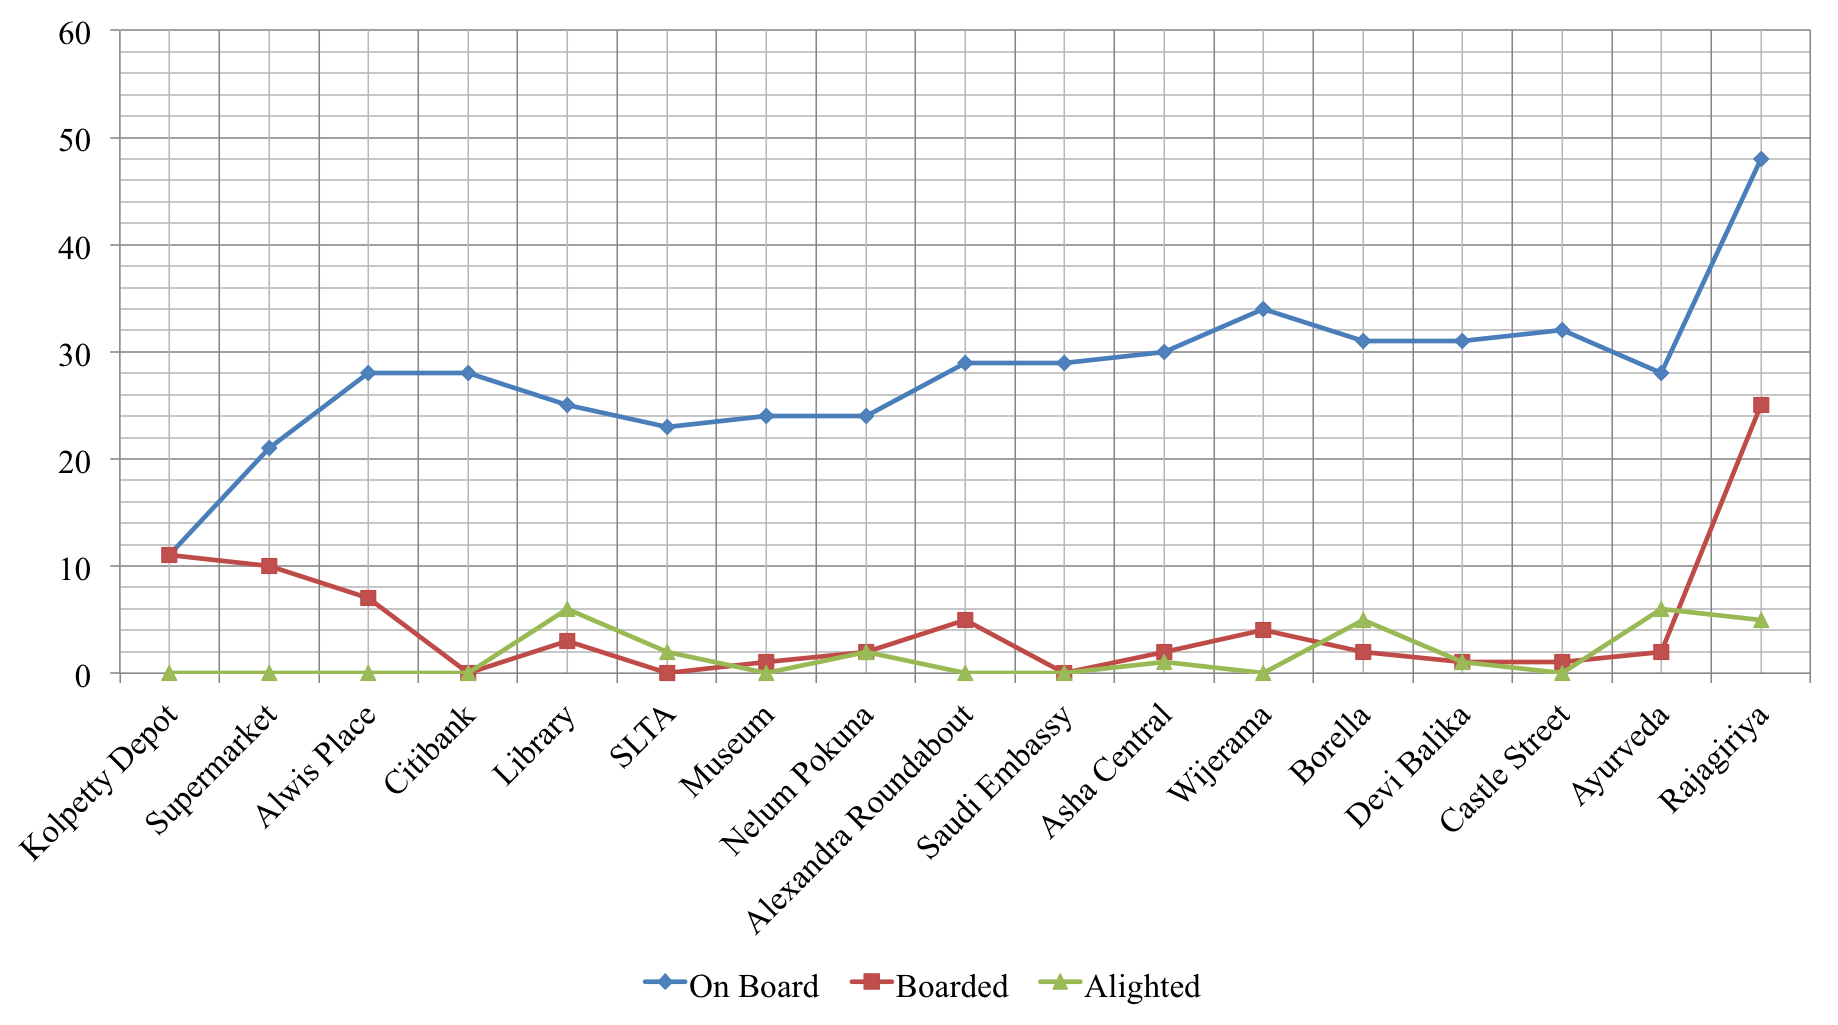
\includegraphics[scale=0.5]{passengerLoadData-Trip1}
\caption [Graph - Passenger Load Fluctuations - Trip 1] {Graph - Passenger Load Fluctuations - Trip 1}
\label {image-passengerLoadData-Trip1}
\end {figure}

\begin {figure} [h!]
\centering
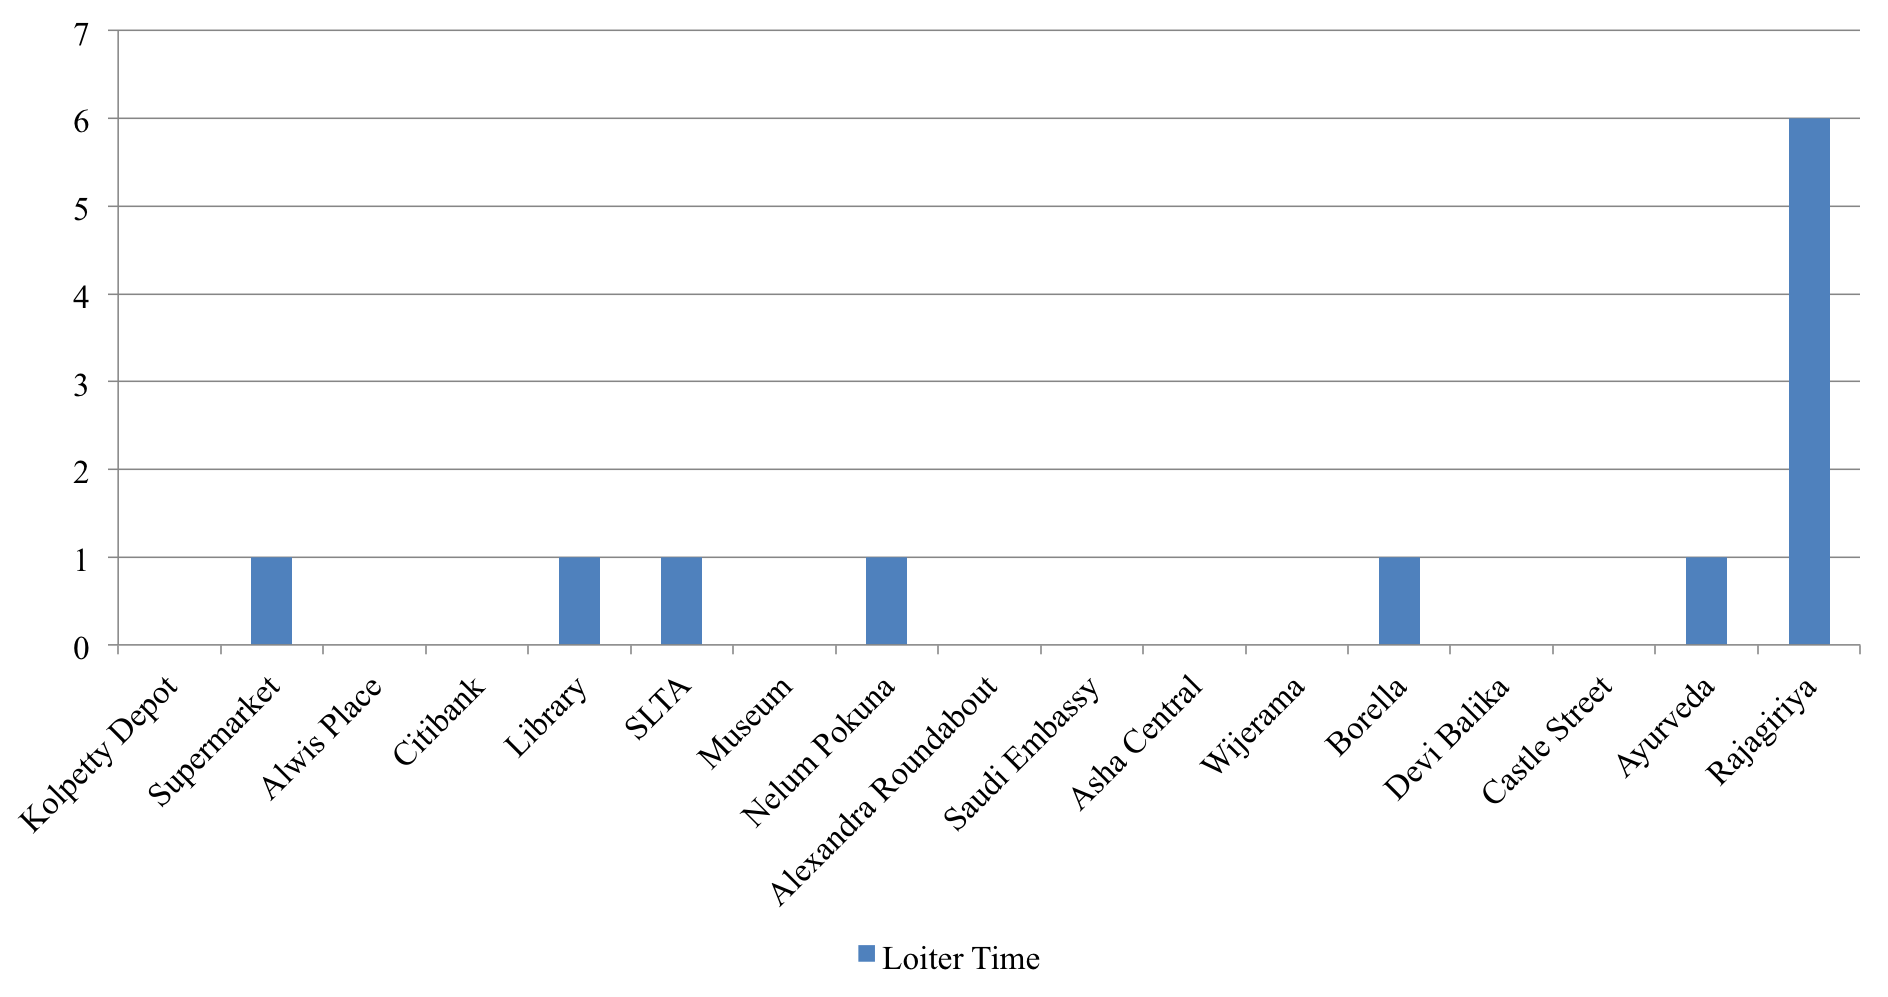
\includegraphics[scale=0.5]{loiterTimeData-Trip1}
\caption [Graph - Bus Loiter Time Data - Trip 1] {Graph - Bus Loiter Time Data - Trip 1}
\label {image-loiterTimeData-Trip1}
\end {figure}

\end{itemize}


\newpage

\section {Stakeholder Analysis}
\label {StakeholderAnalysis}

\paragraph{} The stakeholders of this Public Transport System are illustrated in Figure~\ref{image-stakeholdersDiagram}.

\begin {figure} [h!]
\centering
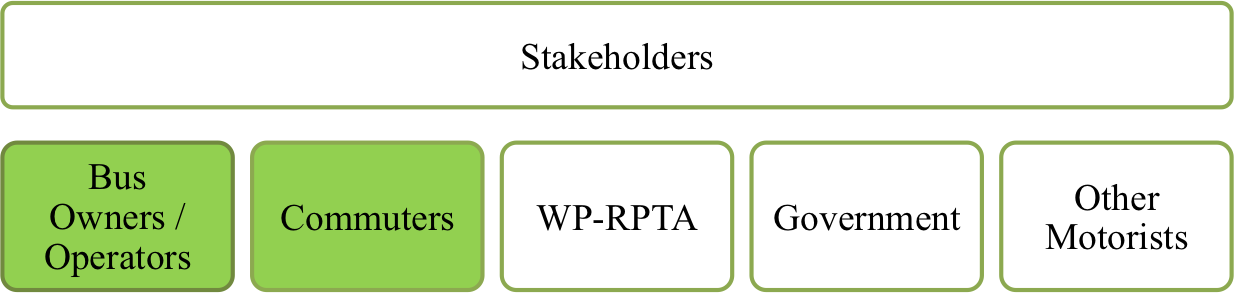
\includegraphics[scale=0.75]{stakeholdersDiagram}
\caption [Stakeholders Diagram] {Stakeholders Diagram}
\label {image-stakeholdersDiagram}
\end {figure}

\paragraph{} The most prominent stakeholders in this system are the Commuters and the Bus Owners/Operators. These 2 serve as the Demand and Supply sides of the economic equation respectively. The conflicting requirements of these two parties are illustrated in Figure~\ref{image-mainStakeholdersDiagram}.

\begin {figure} [h!]
\centering
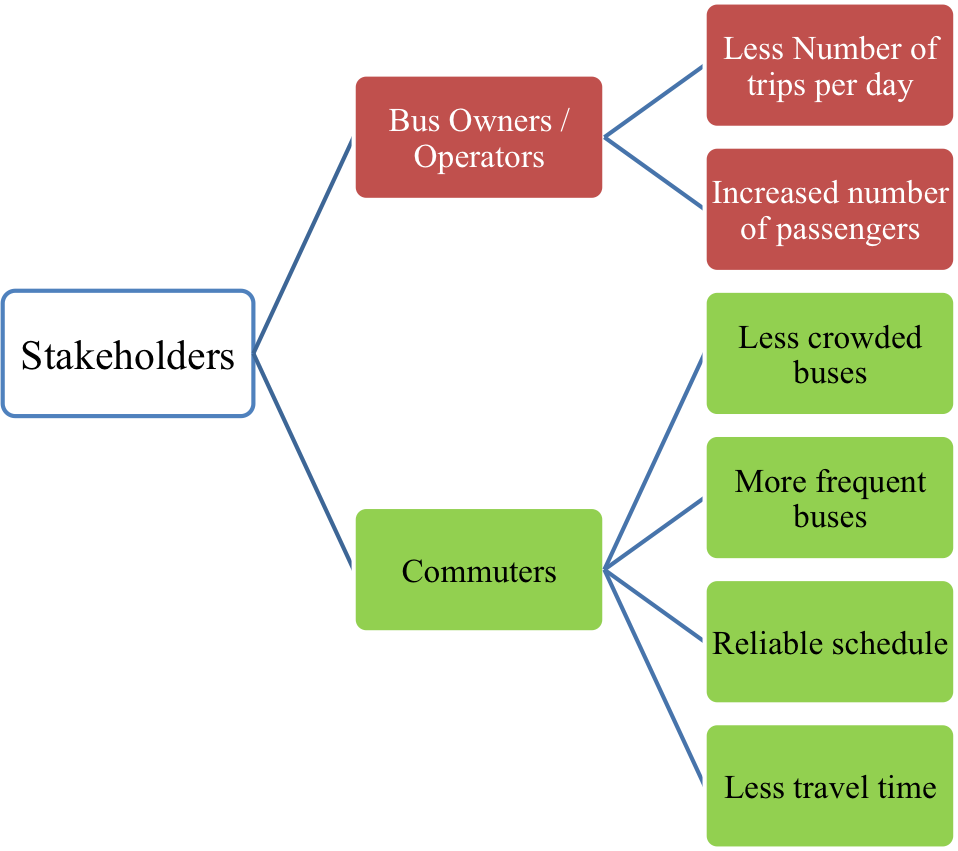
\includegraphics[scale=0.7]{mainStakeholdersDiagram}
\caption [Requirements of Main Stakeholders] {Requirements of Main Stakeholders}
\label {image-mainStakeholdersDiagram}
\end {figure}

\paragraph{} However, it is the Transport Authority that has the responsibility to keep these two parties happy. Therefore the most important stakeholder of the whole system is the Transport Authority and that is why it is important that a System is implemented that assists the Schedulers in their decision-making process. The workflow of the Scheduling Unit of the WP RPTA is comprised of 3 main stages. They are illustrated in Figure~\ref{image-timetablingProcessSteps}. The proposed Decision Support System,detailed in Chapter~\ref{chapter-ProposedSolution} will have this workflow at its core.

\begin {figure} [h!]
\centering
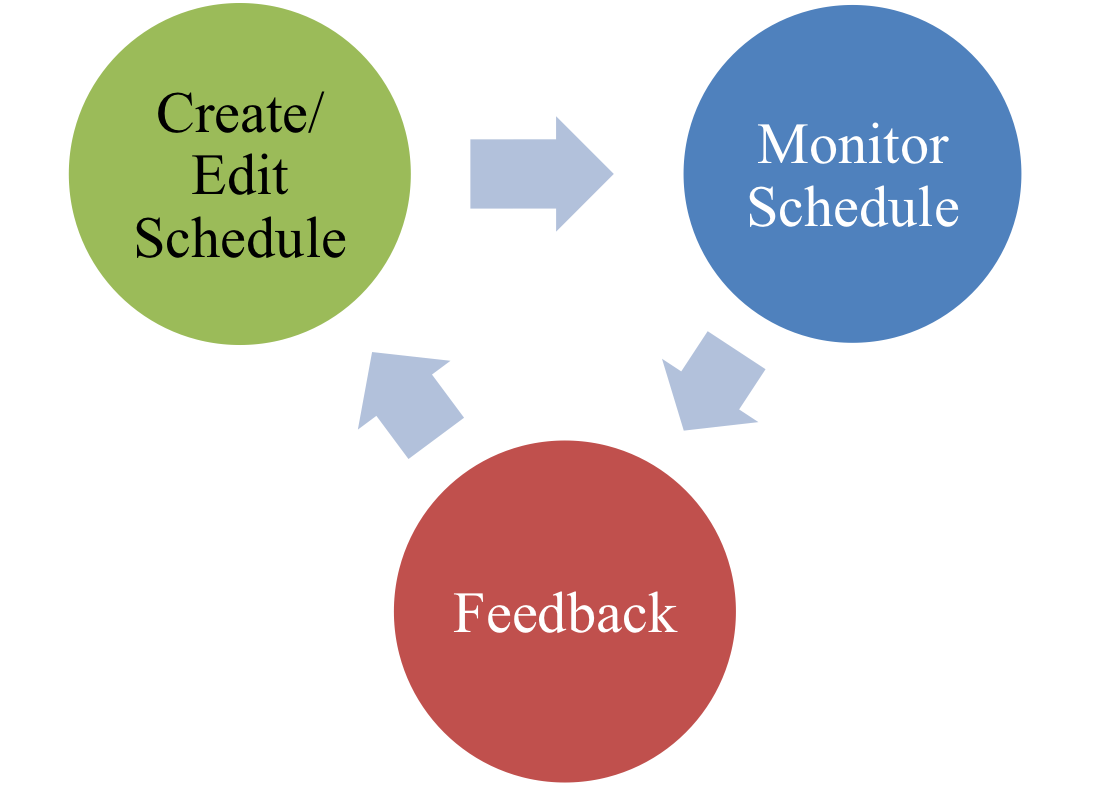
\includegraphics[scale=0.5]{timetablingProcessSteps}
\caption [Stages in the Timetabling Process Flow] {Stages in the Timetabling Process Flow}
\label {image-timetablingProcessSteps}
\end {figure}

\newpage

\section{Possible Alternative Solutions}
\label{section-Alternatives}

\paragraph{} From the contents of the current Chapter, the problems of the current system and transport service are clearly evident. From the Pilot Route Survey that was conducted, the data gathering requirements of the proposed DSS is clear.

Accordingly, possible solutions to these problems were an implementation of a Management Information System or a standalone system to create timetables for the schedulers. However neither of these really addressed all of the issues for all of the stakeholders. Management Information Systems are systems or processes that provide the information necessary to manage an organization effectively \cite{Comptroller1995, TexasAMUni2012}. Although this does accomplish the outcome of better management for the Schedulers, it does little to manage the customer-facing activities. It also focuses on management of the organization instead of aiding in the decision-making process.

Alternatively, a standalone system to merely create timetables and schedules for the bus routes does not solve all of the problems faced. Therefore, the need for a Decision Support System to aid the various stakeholders in their decision-making processes as well as enabling the proper monitoring and regulation of the service is clearly evident. The definition of a Decision Support System and how it relates to the transportation problem has already been discussed in this document. Therefore, in the next Chapter, we will see what the proposed Decision Support System is. This will include the higher-level system architecture, the system features, the main entities \& their relationships and a few screenshots of the prototype that was built for user testing.